\section{Analysis}
A web API (Application Programming Interface) is a set of standard protocols to interact with a web server. This project aims to produce a user-friendly means to interact with the SpaceTraders API.

\subsection{Programming Language}
The first decision to make regarding to this project is that of programming language – more specifically a choice between two stable, statically typed languages with strong module support and asynchronous runtimes. Go and Rust. The former (renowned for its simplicity and concurrency) would offer an expediated development cycle with an extensive standard library. Rust, however, offers memory safety, performance and a strict typing system – enforcing good programming practices. In addition to a superior multiplatform bundler for distributing the program as a single binary without dependencies. Furthermore, Rust has a more mature and documented ecosystem for Terminal User Interfaces (TUI) and Command Line Interfaces (CLI) – which I intend to explore as a means for the user to interact with the API. Below is the same program demonstrating registration with the SpaceTraders API written in Rust and Go respectively to illustrate their differences. 

\begin{lstlisting}[language=C]
use std::collections::HashMap;
use reqwest::{Client, Error};

async fn register() -> Result<String, Error> {
    let client = Client::new();

    let agent = HashMap::from([
        ("symbol", "L30_DESILVA"), 
        ("faction", "COSMIC")
    ]);

    let res = client
        .post("https://api.spacetraders.io/v2/register")
        .header("Content-Type", "application/json")
        .json(&agent)
        .send()
        .await?
        .json::<serde_json::Value>()
        .await?;

    if let Some(error) = res.get("error") {
        println!("{}", error["message"])
    } else {
        println!("Congratulations, {}. You have been 
            registered. Please note your token.", 
            res["data"]["agent"]["symbol"]);
        println!("{}", res["data"]["token"]);
    }

    Ok(res["data"]["token"].to_string());
}

#[tokio::main]
async fn main() {
    let _ = register().await.unwrap();
}

\end{lstlisting}

\begin{lstlisting}
$ http_prototype git:(master): cargo run
    Compiling http_prototype v0.1.0 
      Finished dev [unoptimized] target(s) in 0.51s
      Running `target/debug/http_prototype`

Congratulations, "L30_DESILVA". You have been registered.
Please note your token:
"eyJhbGciO[...]QhEdECLg"

$ http_prototype git:(master): cargo run
    Finished dev [unoptimized] target(s) in 0.07s
     Running `target/debug/http_prototype`

"Cannot register agent. Agent symbol L30_DESILVA has already been claimed." 

\end{lstlisting}

The equivalent Go code, due to its simplicity, can be tedious and lengthy to write. 

\begin{lstlisting}
package main

import (
	"bytes"
	"encoding/json"
	"fmt"
	"net/http"
)

type Register struct {
    Data map[string]interface{}
    Error map[string]interface{}
}

func main() {
    body, err := json.Marshal(map[string]string{
        "symbol": "TRUCKER",
	 "faction": "COSMIC",
    }) 

    if err != nil {
        panic(err)
    }

    req, err := http.NewRequest(
        "POST",       
        "https://api.spacetraders.io/v2/register", 
        bytes.NewBuffer(body)
    )

    if err != nil {
        panic(err)
    }

    req.Header.Add("Content-Type", "application/json")
    client := &http.Client{}
    res, err := client.Do(req)
    if err != nil {
        panic(err);
    }

    defer res.Body.Close()

    data := Register{}
    err = json.NewDecoder(res.Body).Decode(&data)
    if err != nil {
        panic(err)
    }

    if len(data.Error) != 0 {
        fmt.Println(data.Error["message"])
    } else {
        var agent map[string]interface{}
        agentJson, err := json.Marshal(data.Data);
        if err != nil {
            panic(err)
        }

        err = json.Unmarshal(agentJson, &agent);
        if err != nil {
            panic(err)
        }

        fmt.Printf("Congratulations, You've been successfully registered. Please note your access token:\n")
        fmt.Println(agent["token"])
    }
}
\end{lstlisting}

Due to its stability, performance, security and mature, centralised ecosystem I will use rust for this project. Although Rust’s somewhat convoluted approach to asynchronous programming will require careful design considerations as to not introduce bugs. 

\subsection{API}
The core gameplay loop revolves around accepting loans, and performing mining operations to gather the required resources to repay those loans. Credits can then be used to improve your fleet and in turn, increase one's mining capacity – allowing larger loans to be taken for more credits.

The Space Traders API offers HTTP end-points with which programs can access, and in turn: play the open universe trading game. Actions are performed via http requests to the Space Traders server, and such actions can range from locating all available shipyards in a system:
\begin{lstlisting}
    curl 'https://api.spacetraders.io/v2/systems/:systemSymbol/waypoints?traits=SHIPYARD' --header 'Authorization: Bearer INSERT\_TOKEN\_HERE'

\end{lstlisting}
To selling ship cargo:

\begin{lstlisting}
curl --request POST \
 --url 'https://api.spacetraders.io/v2/my/ships/:miningShipSymbol/sell'
 --header 'Authorization: Bearer INSERT_TOKEN_HERE' \
 --header 'Content-Type: application/json' \
 --data '{
    "symbol": "IRON_ORE",
    "units": "100"
   }'
\end{lstlisting}

However, there are 2 versions of the SpaceTraders API in production, the complete V1, and the alpha V2 release. The former is a simpler system, more mature, and has a wider variety of existing frontend clients to learn from. Yet lacks much of the functionality of the second release.  Whereas V2 consists of a larger universe, a wider breadth of features, and comprehensive documentation. Thus, my project will utilise the V2 API specification albeit hesitant of potential bugs due to the alpha nature of its release. 

\subsection{Existing Systems}
There are various existing frontends that use either a command line interface (CLI), or a graphical user interface (GUI) to different effects. A command line interface (as illustrated below) allows for expediated development, however can appear confusing, intimidating, and untintuitive without experience.
\bigskip

\shadowbox{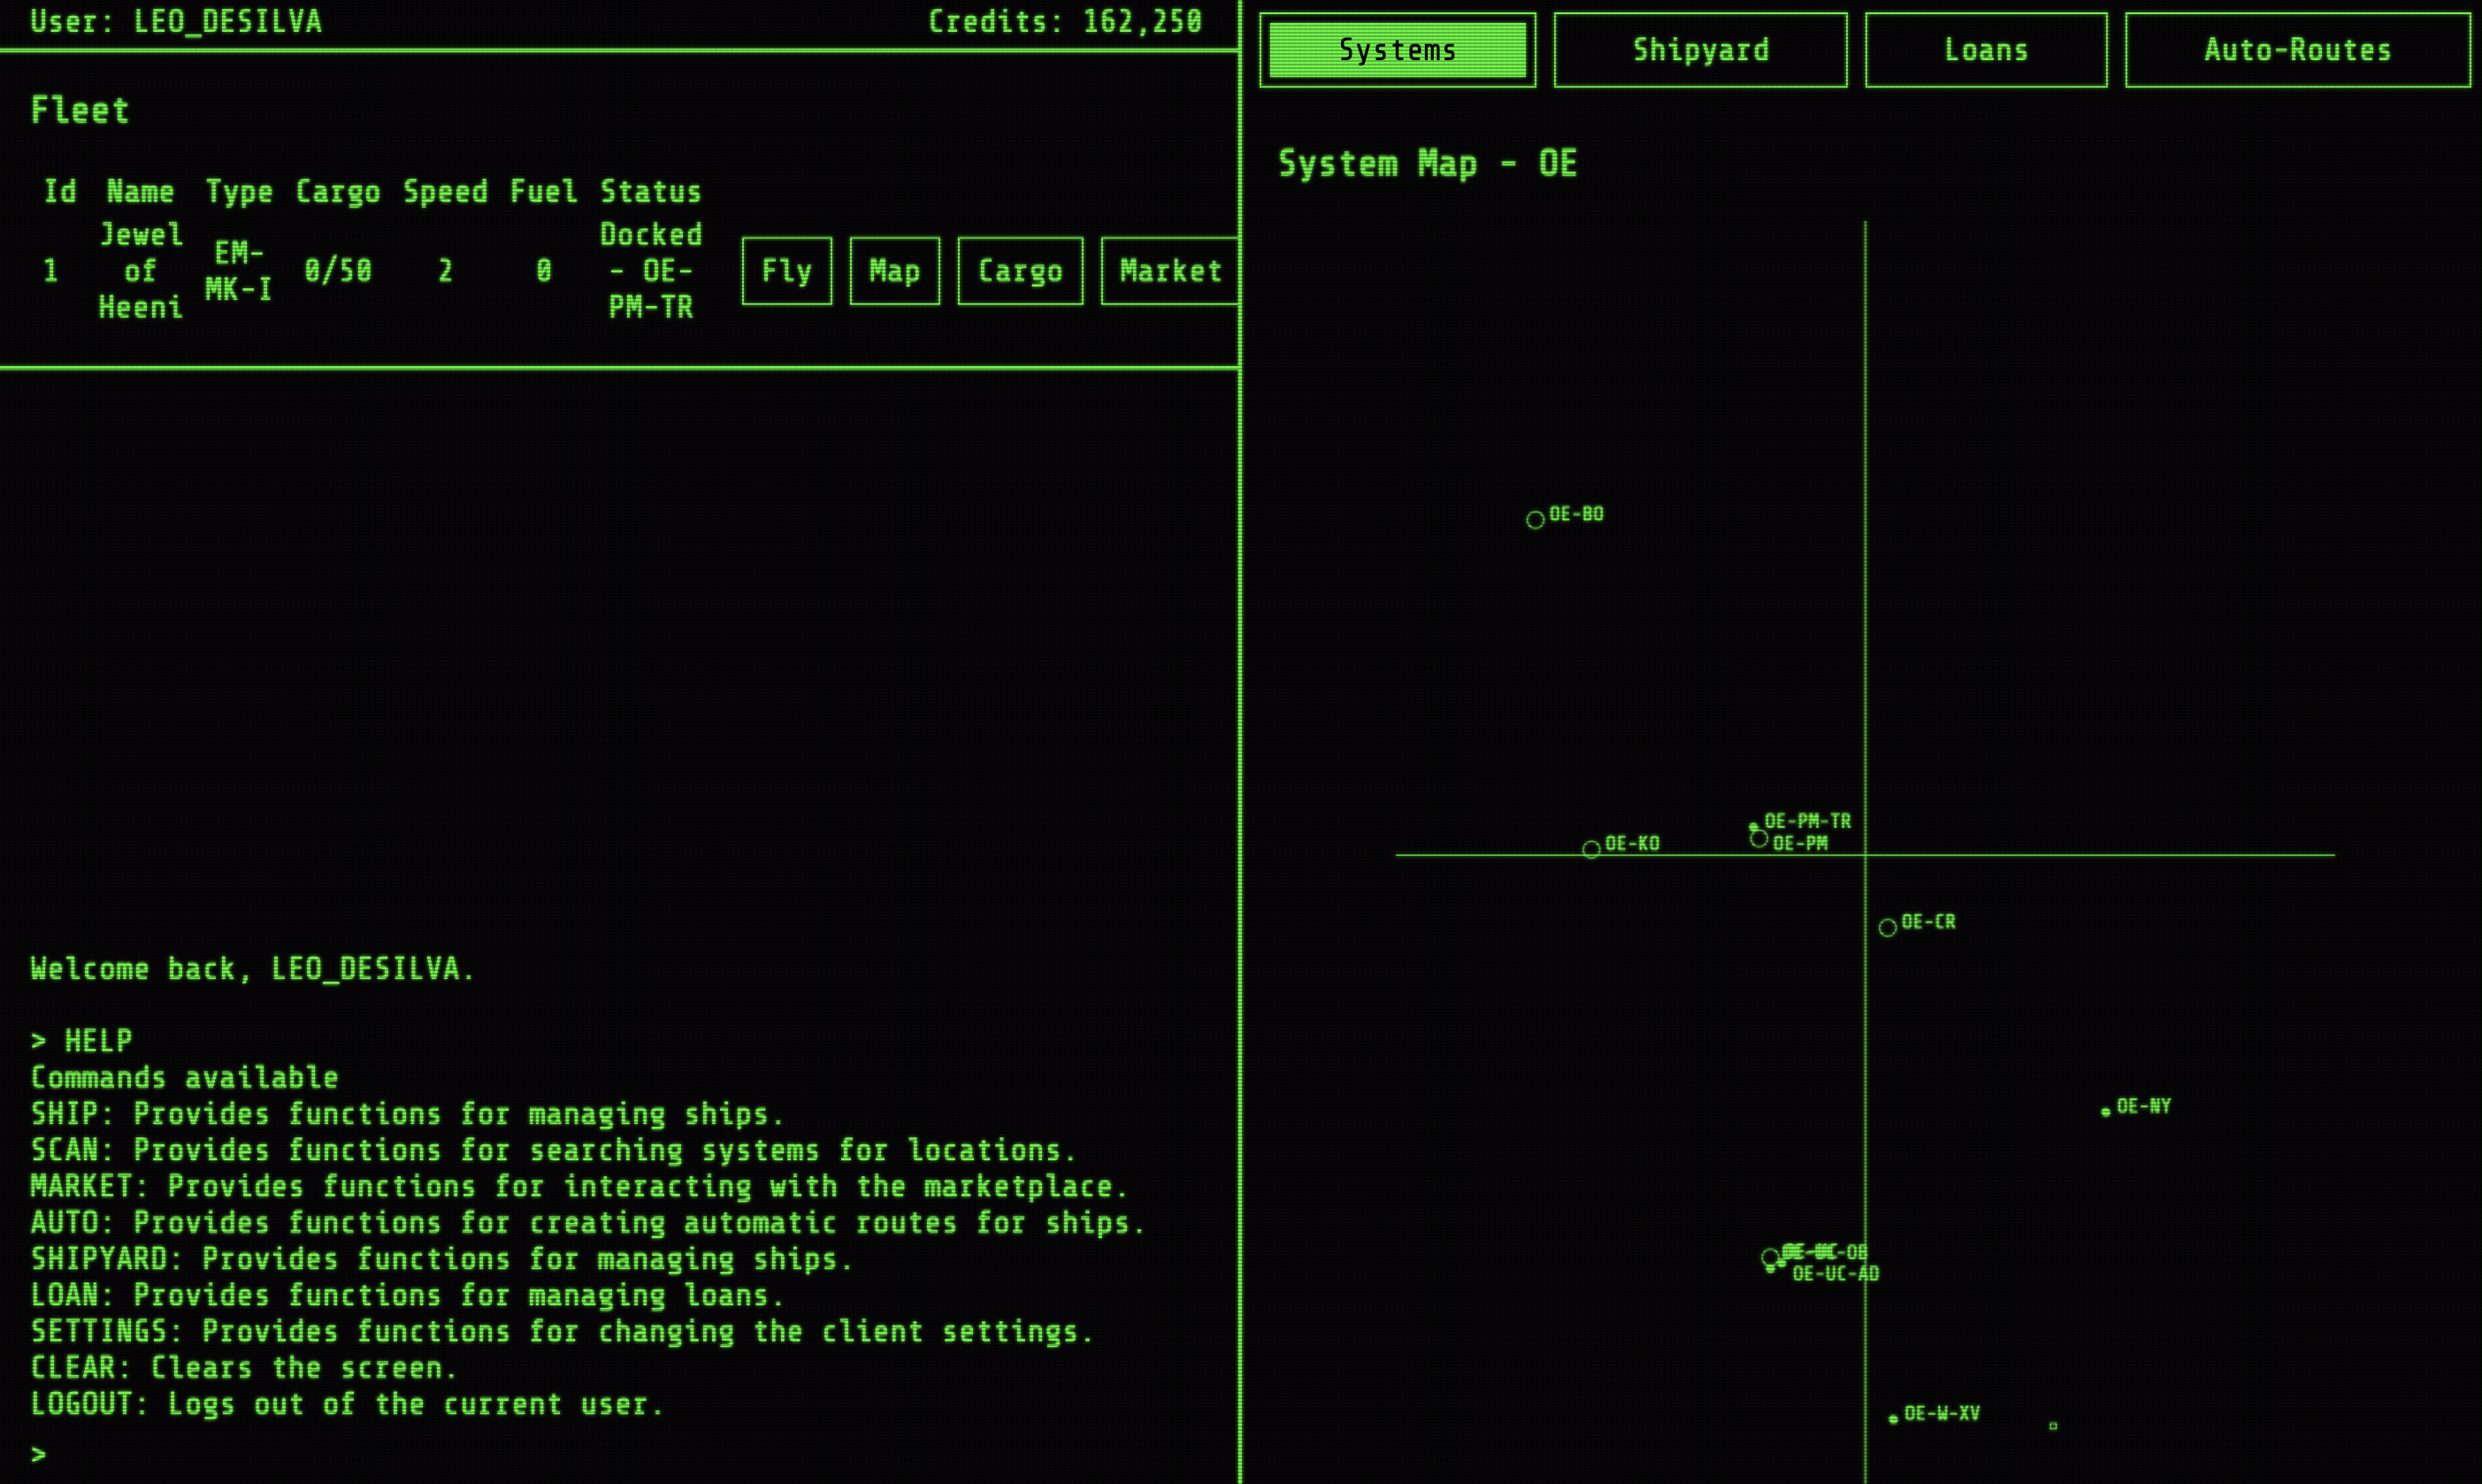
\includegraphics[width=12cm]{trade-commander.png}}



However a GUI provides a visually intuitive experience, \cite{knuthwebsite}offering buttons, icons and menus in place of complex commands and a level of visual feedback that cannot be replicated through a command line. However, GUI development requires significantly more time and resources – often sarcificing flexibility and efficiency for ease of use.

\bigskip
\shadowbox{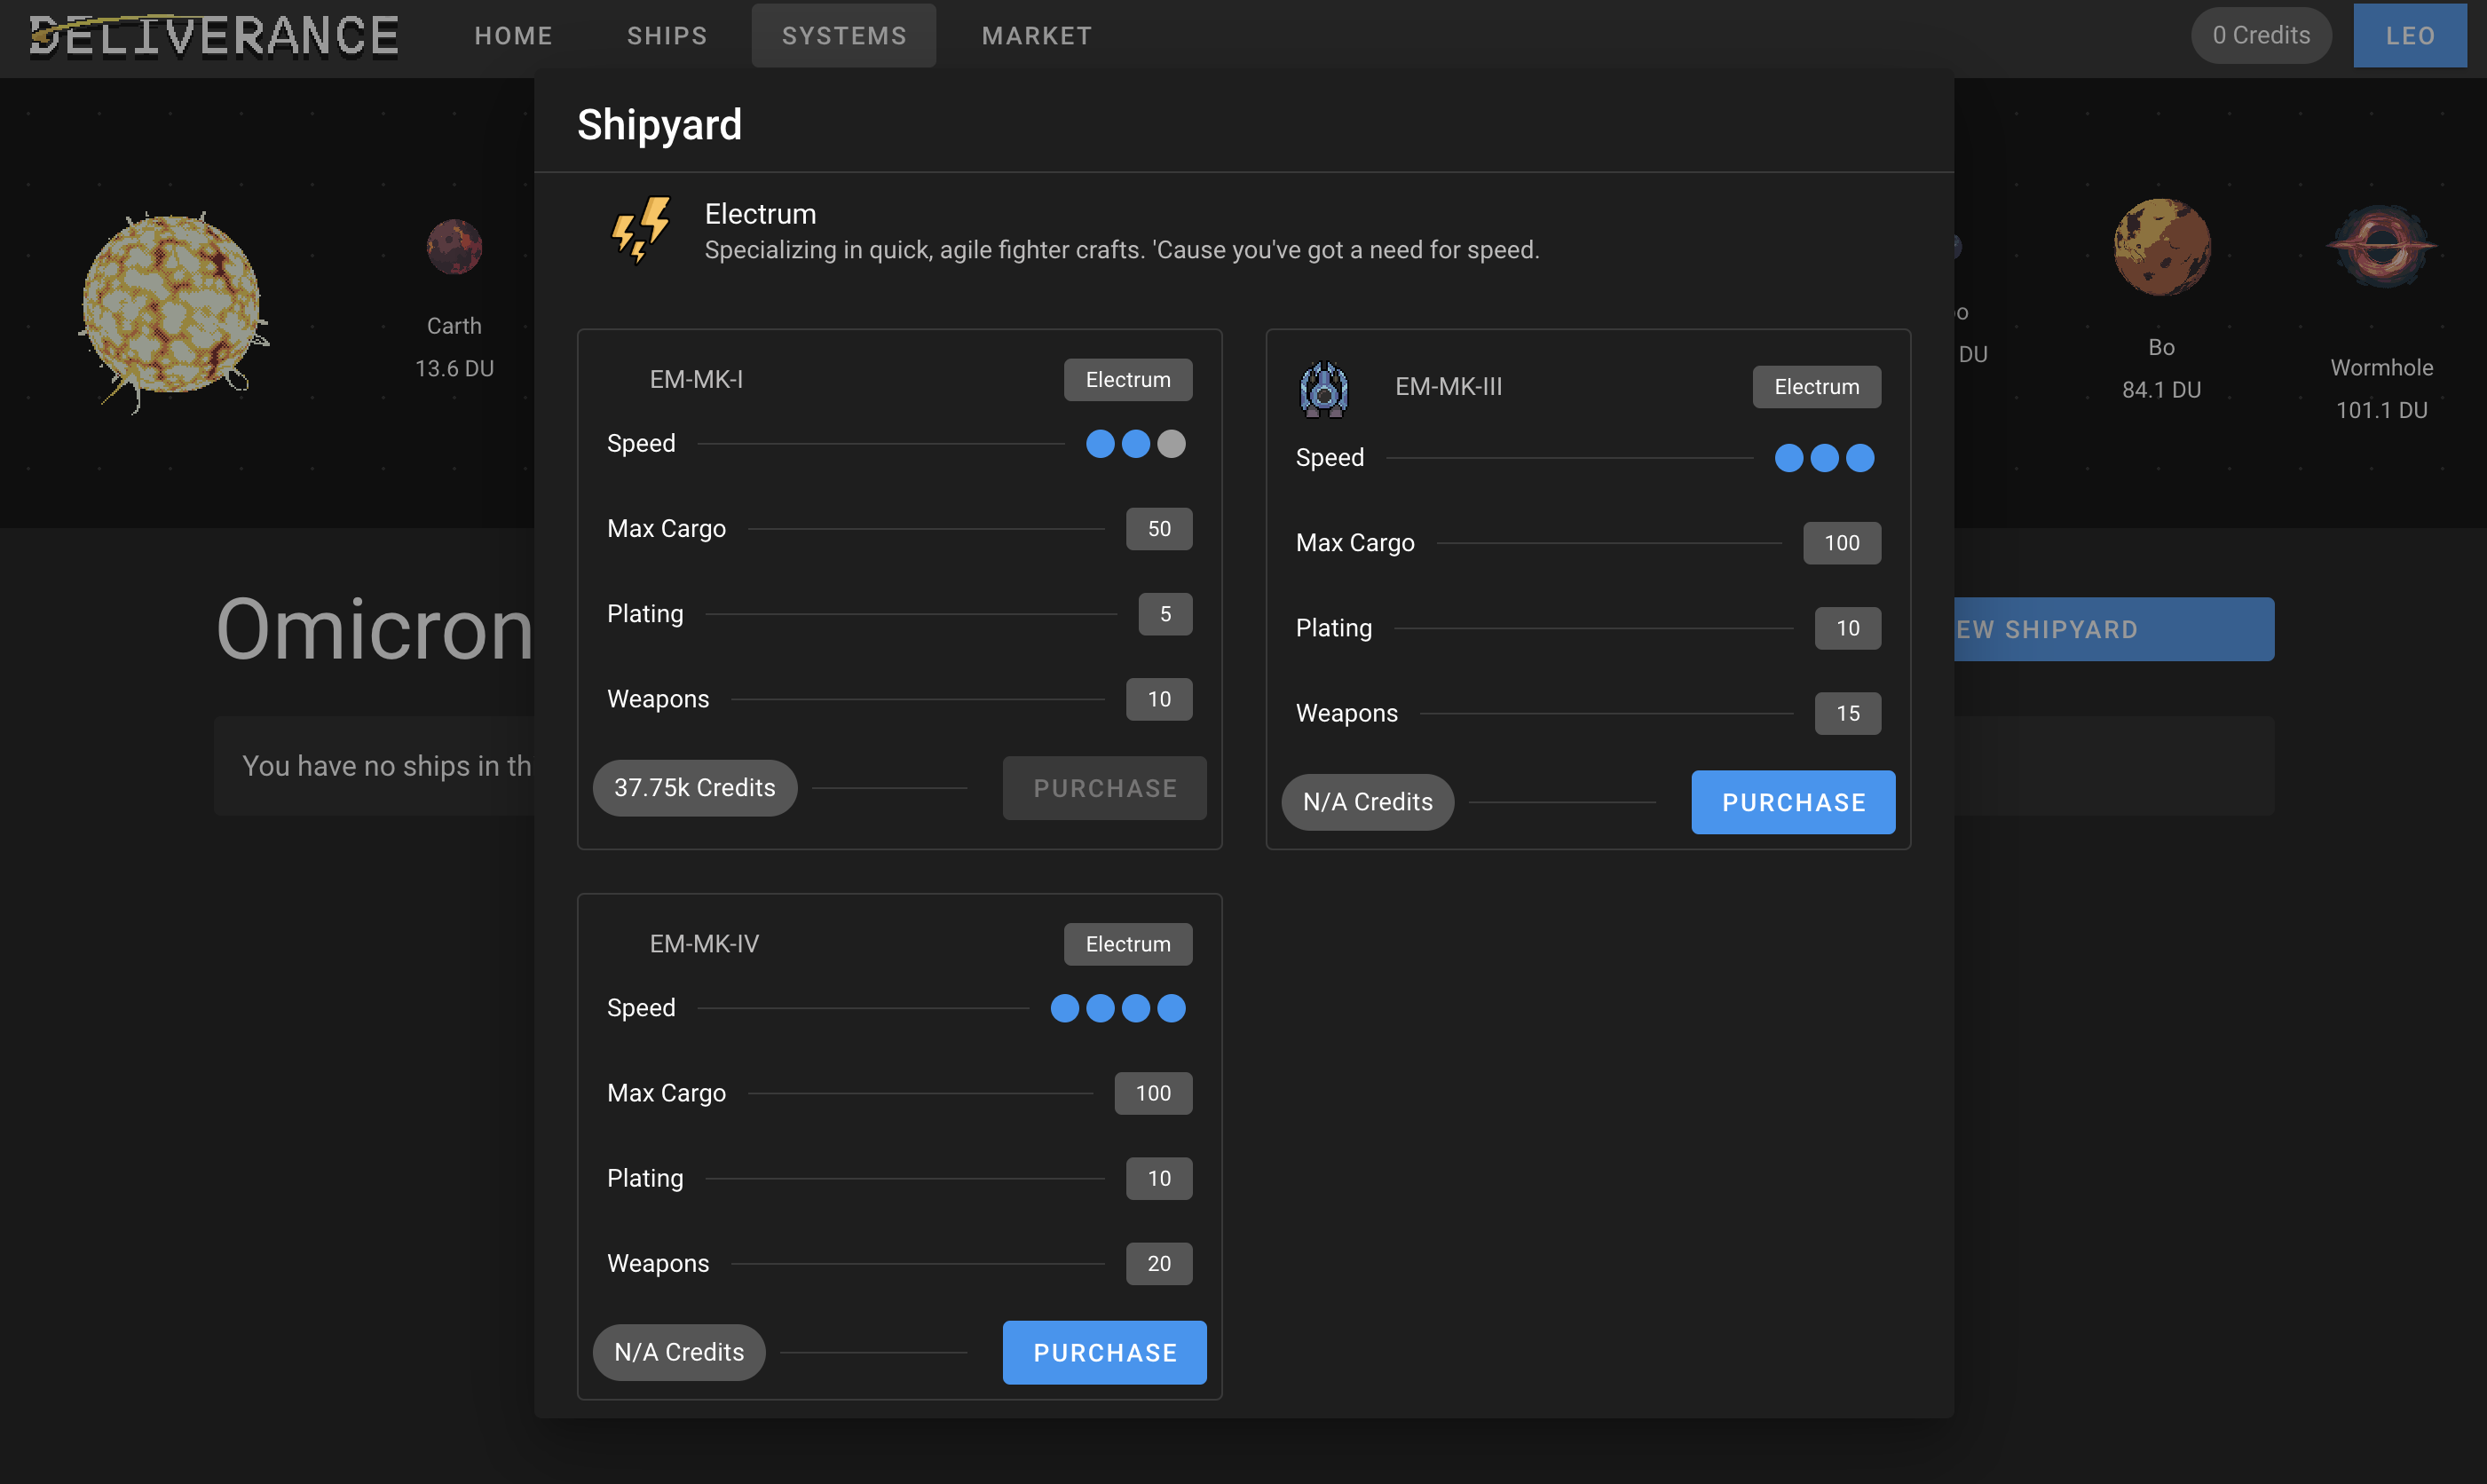
\includegraphics[width=12cm]{deliverance.png}}